\documentclass[notitlepage]{report}

\title{
	\textsc{ \small
		Physics 415
	} \\
	{\textsc{\small Lab \#2}} \\
	Elitzur Vaidman Interaction-free quantum measurement
}
\author{Kevin Evans \\ Partner: Sierra Ray}
\date{February 23, 2021}
\usepackage{amssymb}
\usepackage{mathtools}

\usepackage{amsthm}
\usepackage{amsmath}
\usepackage{slashed}
\usepackage{relsize}
\usepackage{threeparttable}
\usepackage{float}
\usepackage{booktabs}
\usepackage{boldline}
\usepackage{changepage}
\usepackage{physics}
\usepackage[inter-unit-product =\cdot]{siunitx}
\usepackage{setspace}
\usepackage{caption}
\usepackage{subcaption}
\usepackage[makeroom]{cancel}
%\usepackage{pgfplots}

\usepackage{enumitem}
\usepackage{times}
\usepackage{titling} % for titlingpage environment
\usepackage{calligra}
\usepackage{graphicx}
\DeclareMathAlphabet{\mathcalligra}{T1}{calligra}{m}{n}
\DeclareFontShape{T1}{calligra}{m}{n}{<->s*[2.2]callig15}{}
\newcommand{\scriptr}{\mathcalligra{r}\,}
\newcommand{\boldscriptr}{\pmb{\mathcalligra{r}}\,}
\newcommand{\emf}{\mathcal{E}}
\renewcommand{\thesection}{\arabic{section}}

\begin{document}
	\begin{titlingpage}
		\maketitle
		\begin{abstract}
			\noindent A Michelson interferometer was used to reproduce the results of the Elitzur and Vaidman bomb-tester experiment. Here, a photo detector was placed at one port of the interferometer and was adjusted to a central dark fringe. One arm of the interferometer was blocked with a paper, resulting in an increase in detected intensity from \SI{0.0}{\mV} to \SI{0.1}{\mV}. 
			The Michelson interferometer was then readjusted such that a bright fringe appeared at the detector. After blocking one arm of the interferometer, the detector reading dropped from \SI{0.7}{\mV} to \SI{0.1}{\mV}.
			This experiment verifies the results of the Elitzur and Vaidman experiment, which the probability of photon detection at an initially dark detector port increases from $P=0$ to $P=1/4$.
		\end{abstract}
	\end{titlingpage}

	\section{Description of Experiment}
	In this experiment, we will use a Michelson interferometer to reproduce the Elitzur and Vaidman bomb-tester experiment. A Michelson interferometer was constructed on a breadboard with a HeNe laser. At the output of the interferometer, a photodetector was placed and attached to a digital multimeter terminated with a \SI{500}{\ohm} resistor. The experimental setup is shown in Figure \ref{fig:pxl20210211222257140}. The interferometer was intentionally misaligned such that no interference pattern was present and the aperture of the photodetector was adjusted to minimize the effect of ambient room light.
	
	
	Next, the Michelson interferometer was adjusted such that the interference pattern had a central dark fringe. The voltage created by the photodetector was recorded. One interferometer arms was blocked by placing a paper in front of the RM2. The voltage was recorded.
	
	The interferometer was adjusted again, but now with a bright central fringe. The voltage was recorded and an object was placed in front of RM2, and the voltage was recorded again.
	
	\begin{figure}[h]
		\centering
		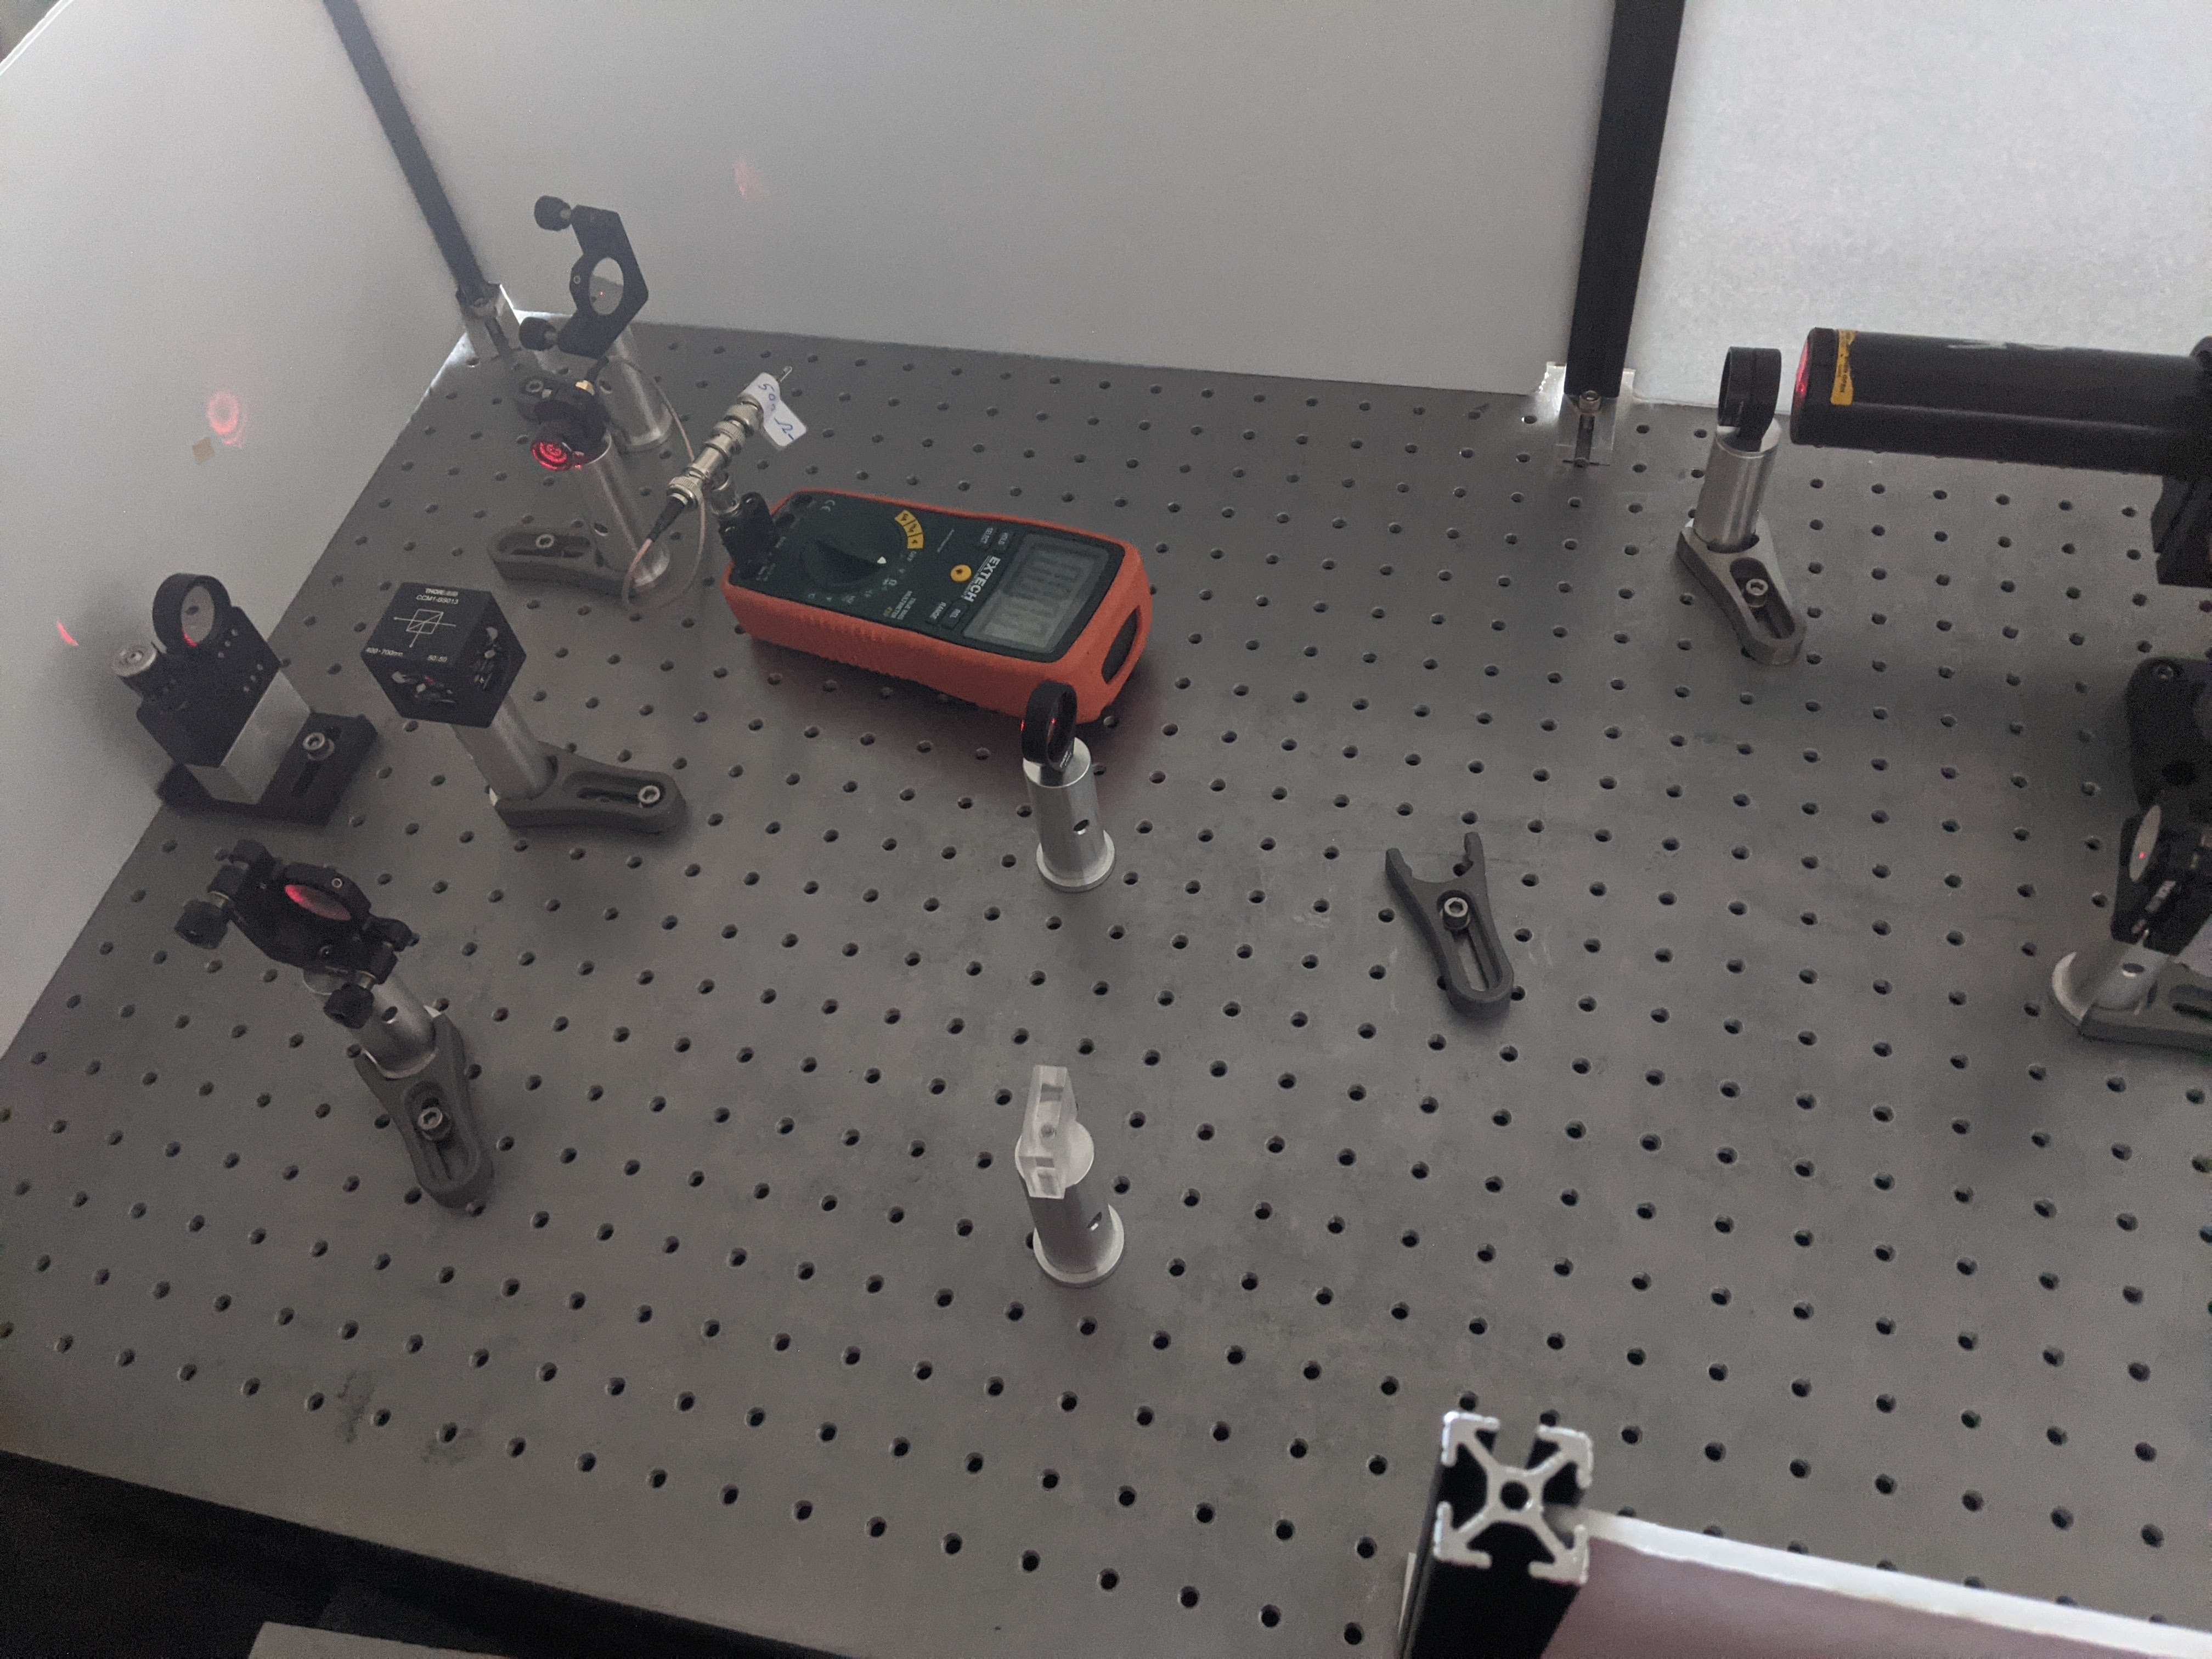
\includegraphics[width=0.7\linewidth]{PXL_20210211_222257140}
		\caption{The Michelson interferometer with photo detector.}
		\label{fig:pxl20210211222257140}
	\end{figure}
	
	
	\section{Data and Analysis}
	The photodiode was placed $\SI{8.9}{\centi\meter} \pm \SI{0.05}{\centi\meter}$ from the beamsplitter cube. The initial intensity reading from the unfocused interference pattern was \SI{0.3}{\mV}. As the unfocused measurement is roughly the average between the bright and dark fringe, we would expect this to be half of the maximum intensity. The maximum voltage is expected to read \SI{0.6}{\V}.
	
	After adjusting the mirrors such that a dark fringe appeared on the photodetector, a voltage of \SI{0.0}{\mV} was found. After blocking the path between the beamsplitter and RM2, the voltage increased between \num{0.1} and \SI{0.2}{\mV}.
	
	Next, the mirrors were adjusted such that a bright fringe appeared on the photodetector. The voltage was found to be \SI{0.7}{\mV}. Blocking the arm reduced the voltage to \SI{0.1}{\mV}.
	
	\section{Results and Conclusion}
	Both a dark and bright central fringe can be used to detect if an object is blocking one arm of the interferometer. 
	
	With the initial dark fringe, this port had a probability of $0$ and the secondary port had a probability of $1$. After blocking the arm, we would expect the probability to detect a photon to increase to $1/4$, and this is what we observe: the voltage increases to a level between \num{0.1} and \SI{0.2}{\mV}. In terms of the bomb tester, this means the probability that the bomb was detected without the explosion is $1/4$.
	
	When the initial fringe was bright, this port had a probability of $1$ and would receive the maximum intensity of light. After the interferometer arm was blocked, the probability must decrease as now there is a probability that the photon would be absorbed by the paper/bomb. It should decrease to $1/4$ and this is similar to what we observe: the intensity level decreases to \SI{0.1}{\mV}.

		

	\section*{Data tables}
	
	\begin{table}[h]
		\caption{Readings of the photodetector.}
		\centering
		\begin{tabular}{lc}
			\toprule
			Description & Voltage (\si{\mV}) )\\
			\midrule
			Unfocused interference pattern & \SI{0.3}{\mV} \\
			Dark fringe & \SI{0.0}{\mV} \\
			Dark fringe, blocked arm & \SI{0.1}{\mV} -- \SI{0.2}{\mV} \\
			Bright fringe & \SI{0.7}{\mV} \\
			Bright fringe, blocked arm & \SI{0.1}{\mV} \\
			\bottomrule
		\end{tabular}
	\end{table}
\end{document}